	\paragraph{QuizziPedia::Front-End::ModelViews::TrainingModelView}
	
	\label{QuizziPedia::Front-End::ModelViews::TrainingModelView}
	
	\begin{figure}[ht]
		\centering
		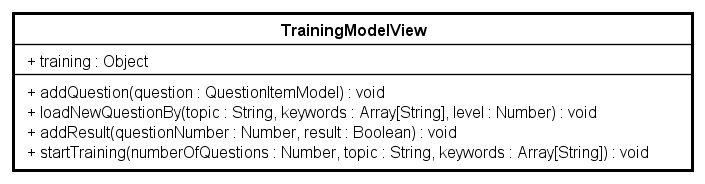
\includegraphics[scale=0.5,keepaspectratio]{UML/Classi/Front-End/QuizziPedia_Front-end_ModelView_TrainingModelView.png}
		\caption{QuizziPedia::Front-End::ModelViews::TrainingModelView}
	\end{figure} \FloatBarrier
	
	\begin{itemize}
		\item \textbf{Descrizione}: classe di tipo modelview la cui istanziazione è contenuta all'interno della variabile di ambiente \texttt{\$scope} di \textit{Angular\ped{G}}. All'interno di essa sono presenti le variabili e i metodi necessari per il \textit{Two-Way Data-Binding\ped{G}} tra la \textit{view\ped{G}} \texttt{TrainingView} e il \textit{controller\ped{G}} \texttt{TrainingController};
		\item \textbf{Utilizzo}: viene utilizzata per effettuare il \textit{Two-Way Data-Binding\ped{G}} tra la \textit{view\ped{G}}\\ \texttt{TrainingView} e il \textit{controller\ped{G}} \texttt{TrainingController} rendendo disponibili variabili e metodi;
		\item \textbf{Relazioni con altre classi}: 
		\begin{itemize}
			\item \textbf{OUT \texttt{TrainingView}}: \textit{view\ped{G}} principale della modalità allenamento, conterrà i vari templates di ogni domanda dell'allenamento; 
			\item \textbf{OUT \texttt{TrainingController}}: questa classe permette di gestire la modalità allenamento sottoponendo all'utente le giuste domande adatte al suo livello.
		\end{itemize}
		\item \textbf{Attributi}: 
		\begin{itemize}
			\item \texttt{+ training: Object} \\ Oggetto contenente al suo interno i seguenti campi:
			\begin{itemize}
				\item \texttt{+ argument: String} \\ Attributo contenente l'argomento scelto dall'utente per l'allenamento;
				\item \texttt{+ keywords: Array[String]} \\ Attributo contenente l'\texttt{array} di keywords scelte dall'utente per l'allenamento;
				\item \texttt{+ questionNumber: String} \\ Attributo che rappresenta il numero progressivo della domanda attuale;
				\item \texttt{+ numberOfQuestions: String} \\ Attributo che rappresenta il numero di domande scelte.
			\end{itemize}
		\end{itemize}
		\item \textbf{Metodi}: 
		\begin{itemize}
			\item \texttt{+ addQuestion(question: QuestionItemModel): void} \\
			Metodo che gestisce l'evento per inserire una domanda nella cronologia delle domande. \\
			\textbf{Parametri}:
			\begin{itemize}
				\item \texttt{question: QuestionItemModel} \\
				Parametro contenente un riferimento all'oggetto di tipo \texttt{QuestionItemModel}.
			\end{itemize}
			\item \texttt{+ loadNewQuestionBy(topic: String, keywords: Array[String], \\level: Number): void} \\
			Metodo che emette l'evento per scaricare una nuova domanda in base ai parametri passati. \\
			\textbf{Parametri}:
			\begin{itemize}
				\item \texttt{topic: String} \\
				Parametro contenente l'argomento della domanda;
				\item \texttt{keywords: Array[String]} \\
				Parametro contenente un\texttt{array} di stringhe che rappresenta le keywords scelte per l'allenamento;
				\item \texttt{level: Number} \\
				Parametro contenente il livello dell'utente.
			\end{itemize}
			\item \texttt{+ addResult(questionNumber: Number, result: Boolean): void} \\
			Metodo che gestisce l'evento per inserire il risultato di una domanda nella cronologia delle domande. \\
			\textbf{Parametri}:
			\begin{itemize}
				\item \texttt{questionNumber: Number} \\
				Parametro contenente il numero della domanda risposta;
				\item \texttt{result: Boolean} \\
				Parametro contenente il risultato della domanda risposta.
			\end{itemize}
			\item \texttt{+ startTraining(numberOfQuestions: Number, topic: String, \\keywords: Array[String]): void} \\
			Metodo che gestisce l'evento per iniziare l'allenamento. \\
			\textbf{Parametri}:
			\begin{itemize}
				\item \texttt{numberOfQuestions: Number} \\
				Parametro contenente il numero di domande per l'allenamento;
				\item \texttt{topic: String} \\
				Parametro contenente l'agomento dell'allenamento;
				\item \texttt{keywords: Array[String]} \\
				Parametro contenente \texttt{array} di parole chiave.
			\end{itemize}
		\end{itemize}
	\end{itemize}
	
	